\documentclass[fleqn]{article}
\usepackage{amsmath, amssymb, esdiff}
\usepackage{gensymb}
\usepackage{tikz, pgfplots}
\usepackage{datetime}
\usepackage{ulem}
\usepackage{xcolor}
\usepackage{enumerate}
\setcounter{secnumdepth}{4}
\newcommand\numberthis{\addtocounter{equation}{1}\tag{\theequation}}


%opening
\title{Lecture 3}
\author{}
\date{\formatdate{4}{11}{2014}}

\begin{document}
	
\maketitle
%\setlength{\mathindent}{0pt}

\tableofcontents

\newpage
\section{Friction}

Friction is an adaptive force, which inhibits the\\
Experimentally, it is observed that $(f_{s})_{\text{max}} \propto N$
\begin{align*}
	(f_{s})_{\text{max}} &\dot{=} \mu_s N\\
	f_{k} &\dot{=} \mu_k N
\end{align*}
It is observed that for most pairs of materials, $f_k < f_s$\\
Hence, against an external force $F$, 
\begin{equation*}
	f = 
	\begin{cases}
		F ; F \leq (f_{s})_{\text{max}} \\
		\mu_{k} N ; F > (f_{s})_{\text{max}} \\
	\end{cases}
\end{equation*}

\begin{tikzpicture}

	\draw [->] (0,0) -- (7,0);
	\draw [->] (0,0) -- (0,5);
	\node [left] at (0,5) {a};
	\node [below] at (7,0) {F};
	
	\draw (0,0) -- (3,0);
	\draw (3,1) -- (5,3);
	
	\draw [dotted] (3,0) -- (3,1);
	\node [below] at (3,0) {$(f_{s})_{\text{max}}$};
	
\end{tikzpicture}

\subsection{Body on a rough inclined plane}

%\begin{tikzpicture}
%	
%	\draw (0,0) -- (10,0) -- (0,10);
%	\draw (5,5) rectangle (5,7);
%	
%\end{tikzpicture}

For the body to be in static equilibrium, 
\begin{align*}
	f &\leq  \mu_s N \\
	&\leq \mu_s m g \cos \theta \\
	f &= m g \sin \theta \\
	\therefore m g \sin \theta &\leq \mu_s m g \cos \theta\\
	\therefore \mu_s &\geq \tan \theta 
\end{align*}

\subsection{Two bodies across a pulley}

\begin{align*}
	N &= m_1 g\\
	T &= m_1 a\\
	m_2 g - T &= m_2 a
\end{align*}
Solving the above equations,
\begin{align*}
	m_2 g &= (m_1 + m_2)a\\
	\therefore a &= \dfrac{m_2}{m_1 + m_2} g
\end{align*}

\subsection{Two bodies across 2 pullies}

\begin{align*}
	m_1 g &= N\\
	T_1 &= m_1 a_1\\
	m_2 g - T_2 &= m_2 a_2\\
	T_2 - 2T_1 &= (0)(a_2) = 0\\
	a_2 &= \dfrac{a_1}{a_2}
\end{align*}

\subsection{2 bodies and a pulley in horizontal plane}

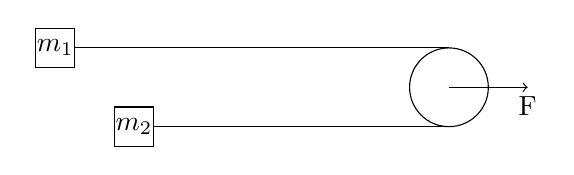
\begin{tikzpicture}
	
	\draw (0,0) circle [radius=0.5];
	
	\draw (-4.75,0.5) -- (0,0.5);
	\draw (-3.75,-0.5) -- (0,-0.5);
	
	\draw (-5.25,0.25) rectangle (-4.75,0.75);
	\node at (-5,0.5) {$m_1$};
	\draw (-4.25,-0.25) rectangle (-3.75,-0.75);
	\node at (-4,-0.5) {$m_2$};
	
	\draw [->] (0,0) -- (1,0);
	\node [below] at (1,0) {F};
	
\end{tikzpicture}

If the pulley moves by a distance $x_3$, $m_1$ moves by $x_1$, and $m_2$ moves by $x_2$. The length of the rope is constant.
\begin{align*}
	\therefore x_1 + x_2 &= 2 x_3\\
	\therefore x_3 &= \dfrac{x_1 + x_2}{2}\\
	\therefore a_3 &= \dfrac{a_1 + a_2}{2}\\
\end{align*}

\subsection{Body on another body with pulley}

\subsubsection{Case I: No relative motion}

\begin{align*}
	(m_1 + m_2)a = F\\
	\therefore a = \dfrac{F}{m_1 + m_2}
\end{align*}

\subsubsection{Case II: Relative motion exists}

\begin{align*}
	m_1 a = \dfrac{F}{2} + f \\
	m_2 a = \dfrac{F}{2} - f \\
\end{align*}

No relative motion will persist as long as 
\begin{equation*}
	f < (f_s)_{\text{max}} = \mu_s N_{12} = \mu_s m_2	
\end{equation*}

\subsection{2 Bodies and 3 pulleys}

For $m_1$,
\begin{align*}
	\hat{y} &: N_{\text{floor}} = m_1 g + T\\
	\hat{x} &: 2T - N = m_1 a_1
\end{align*}
For $m_2$,
\begin{align}
	\hat{y} &: m_2 g - T = m_2 a_2\\
	\hat{x} &: N = m_2 a_1\\
	a_2 &= 2 a_1
\end{align}

\subsection{}

\begin{tikzpicture}
	
	\draw (-5,0) -- (5,0); 
	
	\draw (-2,0) rectangle (2,2);
	\node at (0,1) {$m_2$};
	
	\draw (-1,2) rectangle (1,3);
	\node at (0,2.5) {$m_1$};

	\draw [->] (2,1) -- (4,1);
	\node [right] at (4,1) {$F(t)$};
	
\end{tikzpicture}\\

Given : The force varies as $F = bt ; b>0$, and the coefficients of friction between all surfaces are $\mu_s$, $\mu_k$.

\paragraph*{Stage I: No movement\\}
No movement will occur till $f = \mu_s N_\text{floor} = \mu_s (m_1 + m_2) g$\\
If movement starts at say $t_0$, 
\begin{align*}
	f = F(t_0) &= b t_0\\
	\therefore \mu_s (m_1 + m_2) g &= b t_0\\
	\therefore t_0 &= \dfrac{\mu_s (m_1 + m_2) g}{b}
\end{align*}

\paragraph*{Stage II: $m_1$ and $m_2$ move together\\}

\begin{align*}
	b t - \mu_k N_{\text{floor}} &= (m_1 + m_2) a\\
	\therefore bt - \mu_k (m_1 + m_2) g &= (m_1 + m_2) a\\
	\therefore a &= \dfrac{b}{m_1 + m_2} t - \mu_k g
\end{align*}
For $m_1$,
\begin{align*}
	\hat{x} : f_{12} = m_1 a\\
	\hat{y} : N_{12} = m_1 g
\end{align*}
For $m_2$,
\begin{align*}
	\hat{x} : F - f - f_{12} = m_2 a\\
	\hat{y} : N_{\text{floor}} = N_{12} + m_2 g
\end{align*}
At $t = t_1$,
\begin{equation*}
	f_{12} = \mu_s n_{12} = \mu_s m_1 g\\
\end{equation*}
Therefore,
\begin{equation*}
	t_1 = \dfrac{(\mu_s + \mu_k) g (m_1 + m_2)}{b}
\end{equation*}

\paragraph*{Stage III: $m_1$ and $m_2$ are in relative motion\\}

For $m_1$,
\begin{align*}
	\hat{x} : \mu_k N_{12} = m_1 a_1\\
	\hat{y} : N_{12} = m_1 g
\end{align*}
For $m_2$,
\begin{align*}
	\hat{x} : bt - \mu_k N_{\text{floor}} - \mu_k n_{12} = m_2 a_2\\
	\hat{y} : N_{\text{floor}} = N_{12} + m_2 g
\end{align*}
Therefore,
\begin{align*}
	a_1 &= \dfrac{\mu_k N_{12}}{m_1}\\
	&= \dfrac{\mu_k m_1 g}{m_1}\\
	&= \mu_k g\\
	a_2 &= \dfrac{b}{m_2} t - \dfrac{\mu_k}{m_2} (m_1 g + m_2 g) - \dfrac{\mu_k m_1 g}{m_2}\\
	&= \dfrac{b}{m_2} t - \mu_k g \left( 2 \dfrac{m_1}{m_2} + 1 \right)
\end{align*}

At $t = t_1$,
\begin{align*}
	a_2 &= \dfrac{b}{m_2} t_1 - \mu_k g \left( 2 \dfrac{m_1}{m_2} + 1 \right)\\
	&= \mu_s g + \dfrac{m_1}{m_2} (\mu_s - \mu_k) g\\
\end{align*}
Therefore, for $t > t_1$
\begin{equation*}
	a_2 > a_1
\end{equation*}

\end{document}